\section{Introduction}

% Sketches are widely used
Data sketching algorithms, or \emph{sketches} for short~\cite{Cormode:2017}, have become 
an indispensable tool for high-speed computations over massive datasets in recent years. 
Their applications include a variety of analytics and machine learning use cases, e.g., data aggregation~\cite{Agarwal:2012, KMV}, 
graph mining~\cite{Cohen:2014},  anomaly (e.g., intrusion) detection~\cite{Yang:2018}, real-time data analytics~\cite{DruidHLL},
and online classification~\cite{Tai:2018}.
%For example, sketches are instrumental in big data analytics systems, which ingest vast amounts of multidimensional data, 
%preprocess it, and provide statistical insights (unique element counts, quantile values, etc.) within interactive user experience 
%constraints. 

% What are sketches
Sketches are designed for \emph{stream} settings in which each data item is only processed once. A sketch data structure 
is essentially a succinct (sublinear) summary of a stream that approximates a specific query (unique element count, quantile values, etc.). 
The approximation is typically 
very accurate -- the error drops fast with the stream size~\cite{Cormode:2017}. 

% Sketches today are sequential
Practical sketch implementations have recently emerged in toolkits~\cite{DataSketches}
and data analytics platforms (e.g., PowerDrill~\cite{GoogleHLL:2013}, Druid~\cite{DruidHLL}, Hillview~\cite{VMWareHillview}, and Presto~\cite{PrestoHLL}). 
However, these implementations are not thread-safe, allowing neither
parallel data ingestion nor concurrent queries and updates; concurrent use is prone to exceptions and 
gross estimation errors. Applications using these libraries are therefore required to explicitly protect all sketch API calls by locks~\cite{lee-groups-post, lee-issue}.
%, forcing sequential access.


\begin{figure}[tb]
\setlength{\abovecaptionskip}{0pt}
\setlength{\belowcaptionskip}{0pt}
\setlength\textfloatsep{0pt}
  \begin{center}
    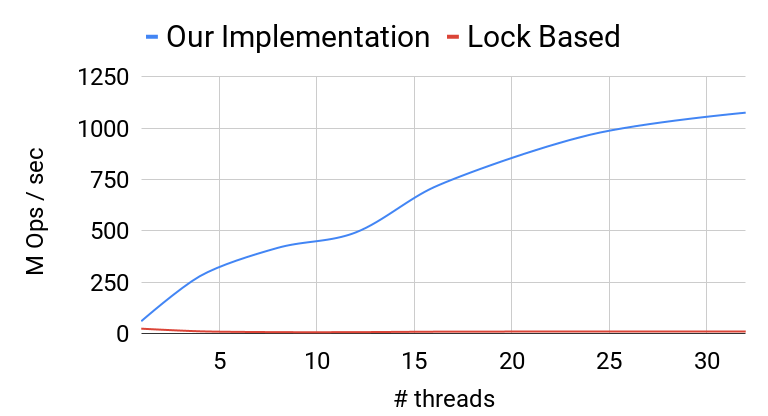
\includegraphics[width=0.39\textwidth]{images/concurrentThetaGraph.png}
  \end{center}
  \caption{Scalability of DataSketches' $\Theta$ sketch 
   protected by a lock vs. our concurrent implementation.}
  \label{fig:performance}
\end{figure}


We present a generic approach to parallelising data sketches efficiently while bounding the error that such a 
parallelisation might introduce. Our goal is to enable simultaneous queries and updates to a sketch from 
multiple  threads. Our solution is carefully designed to do so without slowing down operations as a result of synchronisation.
This is particularly challenging because sketch libraries are extremely fast, often processing tens of millions of updates per second. 

We capitalise on the well-known sketch \emph{mergeability} property~\cite{Cormode:2017}, which enables computing a sketch 
over a stream by merging sketches over substreams. Previous works have exploited this property for distributed 
stream processing (e.g.,~\cite{GoogleHLL:2013, cormode2011algorithms}), devising solutions with a sequential bottleneck at the merge phase and where queries cannot
be served before all updates complete. 
In contrast, our method is based on shared memory and constantly propagates results to a queryable sketch.
We adaptively parallelise  stream processing:  
for small streams, we forgo parallel ingestion as it might introduce significant errors;  
but as the stream becomes large, we process it in parallel using small
thread-local sketches with continuous background propagation of local results to the common (queryable) sketch.

We instantiate our generic algorithm with two popular sketches from the open-source Apache DataSketches 
(Incubating) library~\cite{DataSketches}:  
(1) a KMV $\Theta$ sketch~\cite{KMV}, which estimates the number of unique elements in a stream;
and (2) a Quantiles sketch~\cite{Agarwal:2012} estimating the stream element with a given rank. 
We have contributed the former back to the Apache DataSketches (Incubating) library~\cite{ConcurrentThetaImp}. 
Yet we emphasize that our design is generic and applicable to additional sketches. 

Figure~\ref{fig:performance} compares
the ingestion throughput of our concurrent $\Theta$ sketch to that of a lock-protected sequential sketch,
on multi-core hardware. As expected, the trivial solution does not scale whereas our algorithm scales linearly. 

Concurrency induces an error, and one of the main challenges we address is analysing this additional error.
To begin with, our concurrent sketch is a concurrent data structure, and 
we need to specify its  semantics. We do so using a flavour of 
%\emph{relaxed consistency} due to Henzinger et al.~\cite{Henzinger}    
\emph{relaxed consistency} similar to~\cite{Henzinger, alistarh2018distributionally}    
%specifically, a restricted form of their   \emph{out-of-order} relaxation 
that allows operations to ``overtake'' some other operations.  
Thus, a query may return a result that reflects all but a bounded number of the updates
that precede it. 
While relaxed semantics were previously used for data structures such as stacks~\cite{Henzinger}
and priority queues~\cite{alistarh, rihani2014multiqueues}, we believe that they are a natural fit for data sketches. 
This is because sketches are typically used to summarise streams that  arise from multiple real-world sources  
and are collected over a network with variable delays, and so even if the sketch ensures strict semantics, 
queries might miss some real-world events that occur before them. Additionally, sketches are inherently approximate.
Relaxing their semantics therefore ``makes sense'', as long as it does not excessively increase the expected error.
%Add that the error is addative and not multplicative
If a stream is much longer than the relaxation bound, then indeed the error induced by the relaxation is negligible. But since the error allowed by such
a relaxation is additive, in small streams it may have a large impact. This motivates our adaptive solution, which forgoes relaxing small streams. 

% correctness roadmap: derandomize,  strong serializability, Adversary model,

We proceed to show that our algorithm satisfies relaxed consistency. 
But this raises a new difficulty: 
relaxed consistency is defined with regards to a deterministic specification, whereas sketches are randomised.
We therefore first de-randomise the sketch's behaviour
by delegating the random coin flips to an oracle. We can then relax the resulting sequential specification.
Next, because our concurrent sketch is used within randomised algorithms, 
it is not enough to prove its linearisability. Rather, 
we prove that our generic concurrent algorithm instantiated with sequential sketch $S$
satisfies \emph{strong linearisability}~\cite{Wojciech} with regards to a relaxed sequential specification of the de-randomised $S$.
 

We then analyse the error of the relaxed sketches under random coin flips, with an adversarial scheduler that may delay operations in a
way that maximises the error. We show that our concurrent $\Theta$ sketch's error is coarsely bounded by twice
that of the corresponding sequential sketch. The error of the concurrent Quantiles sketch approaches
that of the sequential one as the stream size tends to infinity.

\vspace{-5pt}
\paragraph{Main contribution} In summary, this paper tackles the problem of concurrent sketches,
offers a general efficient solution for it, and rigorously analyses this solution. While the
paper makes use of many known techniques, it combines them in a novel way.
%we are not aware
%of any previous application of relaxed consistency to randomised statistical algorithms.
%\inred{ We discuss the difficulty of maintaining a bounded error for small streams, and show that this can be overcome without taking away from the overall performance.}
The main technical challenges we address are (1) devising a high-performance generic algorithm 
that supports real-time queries concurrently with updates without inducing an excessive error; 
(2) proving the relaxed consistency of the algorithm; 
and (3) bounding the error induced by the relaxation in both short and long streams.

The paper proceeds as follows:
Section~\ref{sec:model} lays out the model for our work and Section~\ref{sec:background} provides background
on sequential sketches. In Section~\ref{sec:concurrentSketches} we formulate a flavour of relaxed semantics
appropriate for data sketches. Section~\ref{sec:genericAlg} presents our generic algorithm, and
Section~\ref{sec:error-bounds} analyses error bounds. Section~\ref{sec:eval} empirically studies the $\Theta$ sketch's performance
and error with different stream sizes. Finally, Section~\ref{sec:discussion}
concludes. The full paper~\cite{rinberg2019fast}
%The supplementary material
formally proves strong linearisability of our generic algorithm, and
includes some of the mathematical derivations used in our analysis.